\documentclass{article}
\usepackage[hmargin=2cm,bmargin=3cm,tmargin=4.5cm,centering]{geometry}
\usepackage{tikzpagenodes}
\usetikzlibrary{calc}
\usepackage{lmodern}
\usepackage{multicol}
\usepackage{lipsum}
\usepackage{atbegshi}
\usepackage{graphicx}
\usepackage{array}
\usepackage{tabu}

\definecolor{blue}{RGB}{25,25,175}
\newcommand\Header{%
\begin{tikzpicture}[remember picture,overlay]
\fill[blue]
  (current page.north west) -- (current page.north east) --
  ([yshift=50pt]current page.north east|-current page text area.north east) --
  ([yshift=50pt,xshift=-3cm]current page.north|-current page text area.north) --
  ([yshift=10pt,xshift=-5cm]current page.north|-current page text area.north) --
  ([yshift=10pt]current page.north west|-current page text area.north west) -- cycle;
\node[font=\sffamily\bfseries\color{white},anchor=east,
  xshift=-1.5cm,yshift=-1.3cm] at (current page.north east)
  {\fontsize{50}{60}\selectfont COS301 Phase 1};
\end{tikzpicture}%
}
\newcommand\Footer{%
\begin{tikzpicture}[remember picture,overlay]
\fill[blue]
  (current page.south west) -- (current page.south east) --
  ([yshift=-40pt]current page.south east|-current page text area.south east) --
  ([yshift=-40pt,xshift=-3cm]current page.south|-current page text area.south) --
  ([xshift=-5cm,yshift=-10pt]current page.south|-current page text area.south) --
  ([yshift=-10pt]current page.south west|-current page text area.south west) -- cycle;
\node[yshift=0.75cm,font=\ttfamily\bfseries\color{white}] at (current page.south) {\fontsize{20}{24}\selectfont EGGSHELL};
\end{tikzpicture}%
}

\pagestyle{empty}
\AtBeginShipout{\Header\Footer}
\AtBeginShipoutFirst{\Header\Footer}

\begin{document}
\begin{titlepage}
	\centering
	{\scshape\LARGE COS 301 EGGSHELL   \par}
	\vspace{1cm}
	{\scshape\Large PHASE ONE \par}
	\vspace{1.5cm}
	{\huge\bfseries NavUP Proposal\par}
	\vspace{2cm}
	{\Large\itshape  Dawie Pritchard 13104340 \\ Peter Rayner 14001757 \\ Henri-Dawid Haasbroek 15046657 \\ Quinton Swanepoel 15245510 \\ Hendrik van der Mewe 15101283 \\ Barnard van Tonder 15008992 \\ Tshepiso Maleka 13267991\par}
	
\end{titlepage}

\tableofcontents

\newpage
\centering
\section{Introduction}
In this document we will discuss a solution for the concept of the navUP system. Which will allow students to be able to navigate through campus to any lecture hall as fast as possible while taking the least congested route.
\subsection {Purpose}
The sole purpose of this document is to define the requirements of the system as well as the technologies that may ( or may not be used ) to develop this product, as well as different ideas that may be plausible to implement based on difficulty as well as time efficiency. We will try and do an in-depth analysis of the concept of navUP as well as technologies already available for us on campus and technologies we can utilize to implement this product. We will attempt to find the best solution for the product as well as iron out issues that may arise later during the course of the project. 
\subsection {Scope}
Design and implement a mobile application that uses the University of Pretoria's campus wi-fi that will deliver a navigational service to users via their smart devices. The application will be named NavUp. The application should contain all the basic functionalities that are already found in common navigation systems.Other functionality required includes searching, saving and providing directions to a location. A UI(User-Interface) is also required to allow users to interact with the application. It should be usable by different types of users allowing them to enter different kinds of information into the system regarding venues, points of interest, events and activities using multiple types of devices and services. (See References Page)
\subsection{References}
References Pertaining the scope:
COS 301 Software Engineering specification found at www.cs.up.ac.za/courses/COS301
\subsection{Overview}
An in detail overview will be given within the rest of the sections. Including ideas, technologies, charateristics etc.
\newpage
\centering
\section{Overall Description}
\subsection{System Environment}
The NavUP system will have 4  basic mediums in which communication will be spread: \\ 1.Students(Users) \\ 2.Mobile Application User Interface( UI)\\ 3.Campus Wi-Fi Hot Spots \\ 4.GPS 
\subsubsection{Users}
The users will connect to the mobile application through the campus wi-fi, every user will be connected to a particular hotspot. Every connection from a user to a hotspot will be tracked in real time and that information will be used accordingly to monitor how many people are in a certain location.
\subsubsection {Mobile Application User Interface(UI)}
Users will use the UI to select where they want to go as well as selecting the shortest route or the fastest route based on hot-spot connections. The mobile application will then use GPS to locate the user and provide an optimal route.
\subsubsection {Campus Wi-Fi Hot Spots}
The mobile application will keep track as to how many people are logged in and then use GPS to determine how many people are in the vicinity of an area which will also be done using the Wi-Fi hotspot using real time tracking. This will enable users to keep track as to how many people are in a certain location and will allow use to avoid highly congested routes. 
\subsubsection{GPS}
GPS will be used to keep track of users through the mobile application. This will allow users to see where they are currently(even when wi-fi is not available) and allow us to determine what will be the best route for the user to their venue. Every user will also be able to see how many people are in a certain location(hotspots) as well as choose the shortest route or fastest route based on the location of the hotspots.
\subsection {Functional Requirements Specification}
\begin{center}
 \vfill
  \begin{center}    
	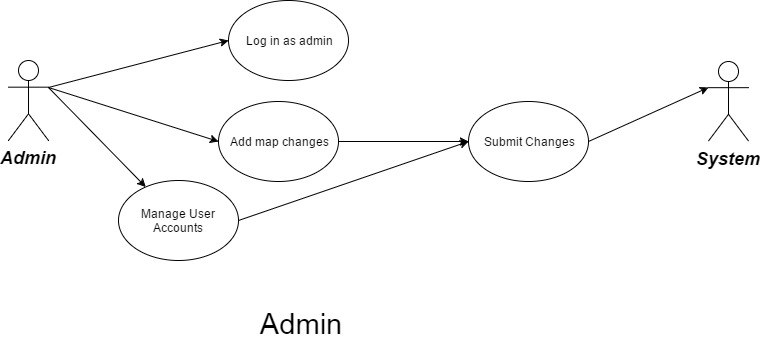
\includegraphics[scale=0.50]{D:/2017-work/INF/Admin.jpg}
  \end{center}
  \vfill
\newpage
 \vfill
  \begin{center}    
	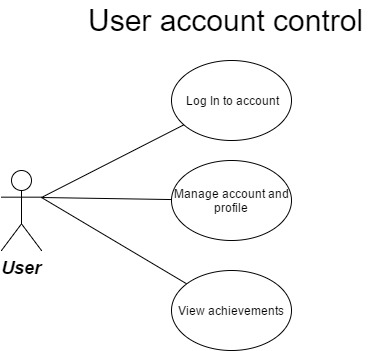
\includegraphics[scale=0.50]{D:/2017-work/INF/UseraccountcontrolV3.jpg}
  \end{center}
  \vfill

\newpage
 \vfill
  \begin{center}    
	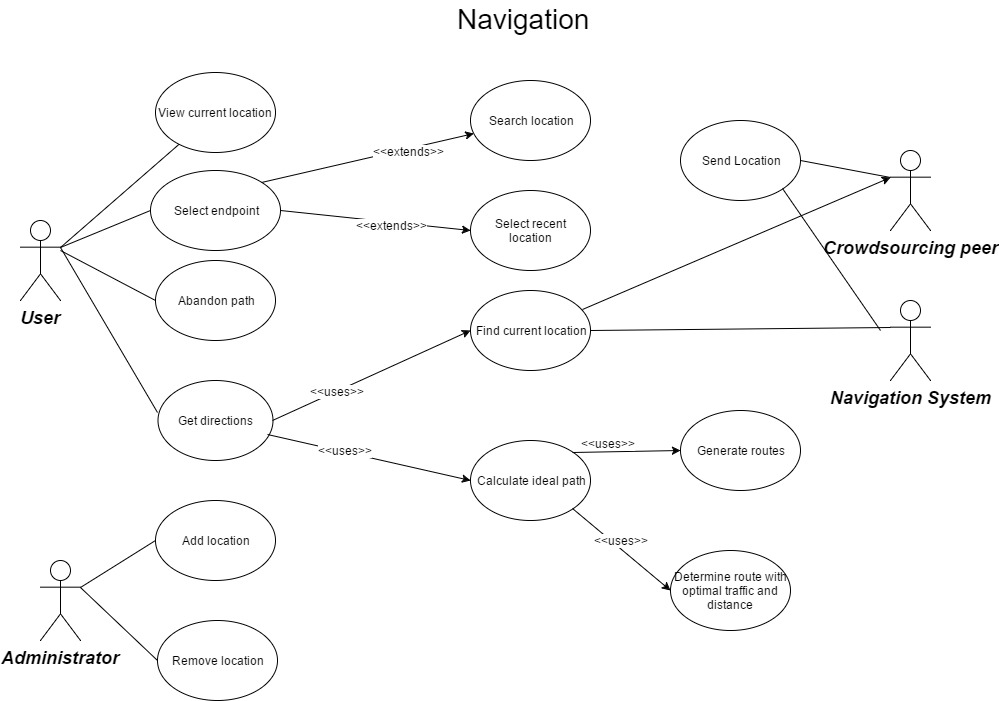
\includegraphics[scale=0.40]{D:/2017-work/INF/NavigateV3 (1).jpg}
  \end{center}
  \vfill

\newpage
 \vfill
  \begin{center}    
	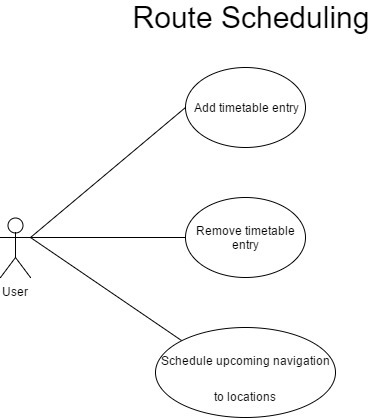
\includegraphics[scale=0.40]{D:/2017-work/INF/SchedulingV3.jpg}
  \end{center}
  \vfill




 \vfill
  \begin{center}    
	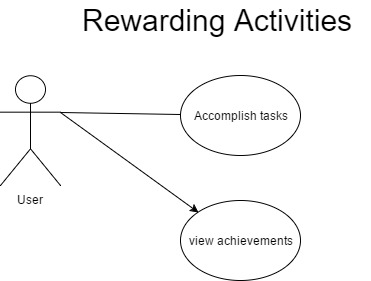
\includegraphics[scale=0.40]{D:/2017-work/INF/ActivitiesV3.jpg}
  \end{center}
  \vfill

\newpage
\centering
\section{Specific Requirements}
\subsection{Functional Requirements}
\subsubsection{Find Location}
The user accesses the mobile application and searches for the location he desires to go too. Pre-Condition: The user needs to be connected to wi-fi and will require the GPS to be activated on the smartphone. Path to locating: Login to app, enable wi-fi, enable GPS, Search location using UI, confirm destination and go to the given location.

\begin{tabu} to 0.8\textwidth { | X[l] | X[c]| }
 \hline

\textbf{use case name} & Find Location \\
 \hline
\textbf{trigger} & User Accesses mobile application    \\
 \hline
\textbf{Precondition} &User has to be connected to Wi-Fi
GPS has to be activated


    \\
\hline
\textbf{Basic Path} & 
\begin{enumerate}
  \item Connect to Wi-Fi network
  \item Activate GPS
  \item Open mobile app
  \item Application determines user location
\end{enumerate}  \\
\hline
\textbf{Alternative Path} & In\textbf{ step 1}, if the user cannot connect to a Wi-Fi network, GPS must be used to determine location
  \newline In \textbf{step 2}, if satellite is down or GPS cannot obtain location, Wi-Fi triangulation is used to determine user location
 \newline  In \textbf{step 4}, if location cannot be determined a message is displayed alerting user that location could not be determined

 \\
\hline
\textbf{Post condition} & Users'' current location displayed   \\
\hline
\textbf{Exception Paths} & None    \\
\hline
\end{tabu}
\newpage
\subsubsection{Update Location}
The users current location is updated whilst moving via real time tracking through the GPS. Pre-Condition: The user needs to be connected to wi-fi and have their GPS activated. Path to locating: Login in to app,enable wi-fi,enable GPS, search location and confirm location.
\begin{tabu} to 0.8\textwidth { | X[l] | X[c]| }
 \hline

\textbf{use case name} & Update Location \\
 \hline
\textbf{trigger} & User location changes    \\
 \hline
\textbf{Precondition} & User has to be connected to the Wi-Fi network
GPS has to activated on the device


    \\
\hline
\textbf{Basic Path} & 
\begin{enumerate}
  \item Connect to Wi-Fi network
  \item Activate GPS
  \item Open mobile app
  \item Find Location
  \item Confirm Location
  \item As user walks to destination, their current location is updated
\end{enumerate}  \\
\hline
\textbf{Alternative Path} & In\textbf{ step 1}, if the user cannot connect to a Wi-Fi network, GPS must be used to determine location
  \newline In \textbf{step 2}, if satellite is down or GPS cannot obtain location, Wi-Fi triangulation is used to determine user location
 \newline  In \textbf{step 4} ,if location cannot be determined a message is displayed alerting user that location could not be determined

 \\
\hline
\textbf{Post condition} & User location updates   \\
\hline
\textbf{Exception Paths} & User may abandon path at any time \\
\hline
\end{tabu}
\newpage

\subsubsection{Add Recently Visited Locations}
When the useer is logged into the application they will have an option to add recently visited locations to their favourite locations. Path to locating: Login to mobile application, go to favourites tab and click on add recent locations.


\begin{tabu} to 0.8\textwidth { | X[l] | X[c]| }
 \hline

\textbf{use case name} & Add Recent Locations \\
 \hline
\textbf{trigger} & User selects option to add location to favourite locations    \\
 \hline
\textbf{Precondition} & User has to be connected to the Wi-Fi network
GPS has to activated on the device
Mobile app has to be open


    \\
\hline
\textbf{Basic Path} & 
\begin{enumerate}
  \item Connect to Wi-Fi network
  \item Activate GPS
  \item Open mobile app
  \item Go to Favourites tab
  \item Click on add recent location
\end{enumerate}  \\
\hline
\textbf{Alternative Path} & If user does not add new locations, system tracks all locations user has navigated to and adds those locations to the  ''Favourites''  list if it is not already in the list


 \\
\hline
\textbf{Post condition} & New recent location added   \\
\hline
\textbf{Exception Paths} & User can abort creation of new recent location     \\
\hline
\end{tabu}
\newpage
\subsubsection{Remove Locations}
The user when logged into the mobile application will have an option to remove recently visited locations from their favourite locations. Path to locating: Login to mobile application. go to favourites tab, click on remove locations.
\newline
\begin{tabu} to 0.8\textwidth { | X[l] | X[c]| }
 \hline

\textbf{use case name} & Remove Location \\
 \hline
\textbf{trigger} & User selects delete option from the Favorites tab    \\
 \hline
\textbf{Precondition} & User has to be connected to the Wi-Fi network
GPS has to activated on the device
Mobile app has to be open


    \\
\hline
\textbf{Basic Path} & 
\begin{enumerate}
  \item Connect to Wi-Fi network
  \item Activate GPS
  \item Open mobile app
  \item Go to ''Favourites'' tab
  \item Click on ''Delete Recent Location''
\end{enumerate}  \\
\hline
\textbf{Alternative Path} & None

 \\
\hline
\textbf{Post condition} & Recent location is removed from ''Favourites'' list   \\
\hline
\textbf{Exception Paths} & None   \\
\hline
\end{tabu}
\newpage
\subsubsection{Track Time to location}
The user will be able to see an estimate time to destination using a timer on the application. Path to locating: Login to mobile application, enable wi-fi, enable GPS, search location, confirm location and time to destination will be visible on the UI. 
\begin{tabu} to 0.8\textwidth { | X[l] | X[c]| }
 \hline

\textbf{use case name} & Time to location \\
 \hline
\textbf{trigger} & User selects location to navigate to    \\
 \hline
\textbf{Precondition} & User has to be connected to the Wi-Fi network
GPS has to activated on the device
Mobile app has to be open
User has to select location to navigate to


    \\
\hline
\textbf{Basic Path} & 
\begin{enumerate}
  \item Connect to Wi-Fi network
  \item Activate GPS
  \item Open mobile app
  \item Search for location
  \item Confirm Location
\end{enumerate}  \\
\hline
\textbf{Alternative Path} & In\textbf{ step 1}, if the user cannot connect to a Wi-Fi network, GPS must be used to determine location
  \newline In \textbf{step 2}, if satellite is down or GPS cannot obtain location, Wi-Fi triangulation is used to determine user location
 \newline  In \textbf{step 4}, if location cannot be found a message is displayed alerting the user that the destination location could not be determined
 \newline  In \textbf{step 5}, if user does not confirm location, estimated time is not displayed

 \\
\hline
\textbf{Post condition} & Estimated time to destination displayed on user interface  


\\
\hline
\textbf{Exception Paths} & User can abort path at any time    \\
\hline
\end{tabu}
\newpage

\subsubsection{Real time tracking of people connected to a wi-fi hotspot-needs checking}
The user will be able to see what path will be the best option based on the tracking of currently connected devices to a certain hot-spot.Path to locating: Login to mobile application, enable wi-fi, enable GPS, search location, confirm route based on hotspot information.
\begin{tabu} to 0.8\textwidth { | X[l] | X[c]| }
 \hline

\textbf{use case name} & Traffic Tracking \\
 \hline
\textbf{trigger} & User selects location to navigate to    \\
 \hline
\textbf{Precondition} & User has to be connected to the Wi-Fi network
GPS has to activated on the device
Mobile app has to be open
User has to select location to navigate to

    \\
\hline
\textbf{Basic Path} & 
\begin{enumerate}
  \item Connect to Wi-Fi network
  \item Activate GPS
  \item Open mobile app
  \item Search for location
  \item Hotspot information retrieved and displayed on routes
  \item User confirms route based on hotspot information
\end{enumerate}  \\
\hline
\textbf{Alternative Path} & In\textbf{ step 1}, if the user cannot connect to a Wi-Fi network, GPS must be used to determine location
  \newline In \textbf{step 2}, if satellite is down or GPS cannot obtain location, Wi-Fi triangulation is used to determine user location
 \newline  In \textbf{step 4}, if location cannot be found a message is displayed alerting the user that the destination location could not be determined
\newline  In \textbf{step 5}, if hotspot information cannot be retrieved, application displays message alerting user that the hotspot information could not be retrieved and possible routes are shown

 \\
\hline
\textbf{Post condition} & Hotspot information displayed to user on all possible routes   \\
\hline
\textbf{Exception Paths} & User may abort location confirmation
User may abort navigation at any time
    \\
\hline
\end{tabu}
\newpage
\subsubsection{Suggest Locations}
The mobile application will be able to suggest Locations based by tracking your daily movements.Path to locating: login to mobile application, visible on home screen

\begin{tabu} to 0.8\textwidth { | X[l] | X[c]| }
 \hline

\textbf{use case name} & Suggest Location \\
 \hline
\textbf{trigger} & User enters application    \\
 \hline
\textbf{Precondition} & User has to be connected to the Wi-Fi network
GPS has to activated on the device
Mobile app has to be open


    \\
\hline
\textbf{Basic Path} & 
\begin{enumerate}
  \item Connect to Wi-Fi network
  \item Activate GPS
  \item Open mobile app
  \item Select Time Tables tab
  \item Suggestions for destinations are displayed to the user
\end{enumerate}  \\
\hline
\textbf{Alternative Path} & None

 \\
\hline
\textbf{Post condition} & Suggested locations displayed to user  \\
\hline
\textbf{Exception Paths} & None   \\
\hline
\end{tabu}
\newpage
\subsubsection{Update path based on traffic of students}
The wi-fi tracking may change whilst a path has already been generated, it will then automatically update the path whilst you are walking.
\begin{tabu} to 0.8\textwidth { | X[l] | X[c]| }
 \hline

\textbf{use case name} & Update path \\
 \hline
\textbf{trigger} & Better alternate route is calculated while navigating to destination   \\
 \hline
\textbf{Precondition} & User has to be connected to the Wi-Fi network
GPS has to activated on the device
Mobile app has to be open
User has to select location to navigate to
User has to confirm destination
User has to be busy navigating to destination


    \\
\hline
\textbf{Basic Path} & While navigating the application measured hotspot traffic on route and redirects user if better path is found with less traffic \\
\hline
\textbf{Alternative Path} & If not better path is found route remains unchanged

 \\
\hline
\textbf{Post condition} & Path is updated and user is redirected  \\
\hline
\textbf{Exception Paths} & None  \\
\hline
\end{tabu}
\newpage
\subsubsection{Generate path to location}
The GPS will acquire the users current location and destination and will generate a path between the two.
\begin{tabu} to 0.8\textwidth { | X[l] | X[c]| }
 \hline

\textbf{use case name} & Generate Path \\
 \hline
\textbf{trigger} & User selects destination    \\
 \hline
\textbf{Precondition} & User has to be connected to the Wi-Fi network
GPS has to activated on the device
Mobile app has to be open
User has to select location to navigate to


    \\
\hline
\textbf{Basic Path} & 
\begin{enumerate}
  \item Connect to Wi-Fi network
  \item Activate GPS
  \item Open mobile app
  \item Search for location
  \item Select location
\end{enumerate}  \\
\hline
\textbf{Alternative Path} & In\textbf{ step 1}, if the user cannot connect to a Wi-Fi network, GPS must be used to determine location
  \newline In \textbf{step 2}, if satellite is down or GPS cannot obtain location, Wi-Fi triangulation is used to determine user location
 \newline  In \textbf{step 4}, if location cannot be found a message is displayed alerting the user that the destination location could not be determined

 \\
\hline
\textbf{Post condition} & Path is generated between users current location and destination and path is displayed to the user \\
\hline
\textbf{Exception Paths} & Select location process can be aborted at any time   \\
\hline
\end{tabu}
\newpage
\subsubsection{Add timetable to mobile application}
The mobile application will have a timetable feature which will enable the app to automatically generate paths from certain locations based on the users individual timetable. 
\begin{tabu} to 0.8\textwidth { | X[l] | X[c]| }
 \hline

\textbf{use case name} & Add Time Table \\
 \hline
\textbf{trigger} & User selects option to add time table    \\
 \hline
\textbf{Precondition} & User has to be connected to the Wi-Fi network
GPS has to activated on the device
Mobile app has to be open


    \\
\hline
\textbf{Basic Path} & 
\begin{enumerate}
  \item Connect to Wi-Fi network
  \item Activate GPS
  \item Open mobile app
  \item Select Time Tables tab
  \item Select Add Time Table
  \item User adds classes to Time Table
\end{enumerate}  \\
\hline
\textbf{Alternative Path} & In\textbf{ step 1}, if the user cannot connect to a Wi-Fi network, GPS must be used to determine location
  \newline In \textbf{step 2}, if satellite is down or GPS cannot obtain location, Wi-Fi triangulation is used to determine user location


 \\
\hline
\textbf{Post condition} & User adds time table and user interface is updated  \\
\hline
\textbf{Exception Paths} & User can abort the add time table process at any time
User can abort add class process at any time
    \\
\hline
\end{tabu}
\newpage
\subsubsection{Remove timetable to mobile application}
The mobile application will let the user remove their own individual timetable based on each semester, or a mistake made.
\newline
\begin{tabu} to 0.8\textwidth { | X[l] | X[c]| }
 \hline

\textbf{use case name} & Remove Time Table \\
 \hline
\textbf{trigger} & User selects option to remove time table    \\
 \hline
\textbf{Precondition} & User has to be connected to the Wi-Fi network
GPS has to activated on the device
Mobile app has to be open
A Time Table has to exist

    \\
\hline
\textbf{Basic Path} & 
\begin{enumerate}
  \item Connect to Wi-Fi network
  \item Activate GPS
  \item Open mobile app
  \item Select Time Tables tab
  \item Select Remove Time Table
  \item User Removes Time Table
\end{enumerate}  \\
\hline
\textbf{Alternative Path} & In\textbf{ step 1}, if the user cannot connect to a Wi-Fi network, GPS must be used to determine location
  \newline In \textbf{step 2}, if satellite is down or GPS cannot obtain location, Wi-Fi triangulation is used to determine user location
 \newline  In \textbf{step 5}, if there are no Time Tables a message will notify user that no Time Tables exist

 \\
\hline
\textbf{Post condition} & Time Table is removed and user interface is updated   \\
\hline
\textbf{Exception Paths} & User can abort the remove time table process at any time    \\
\hline
\end{tabu}
\newpage
\subsubsection{Voice Input for location}
Users will be able to use voice input when trying to access a certain location.
\begin{tabu} to 0.8\textwidth { | X[l] | X[c]| }
 \hline

\textbf{use case name} & Voice Input for location \\
 \hline
\textbf{trigger} & User select option to input location by means of voice recognition    \\
 \hline
\textbf{Precondition} & User has to be connected to the Wi-Fi network
GPS has to activated on the device
Mobile app has to be open

    \\
\hline
\textbf{Basic Path} & 
\begin{enumerate}
  \item Connect to Wi-Fi network
  \item Activate GPS
  \item Open mobile app
  \item Select “Say Destination Name” button
  \item User  says the name of destination
  \item Destination location is retrieved
\end{enumerate}  \\
\hline
\textbf{Alternative Path} & In\textbf{ step 1}, if the user cannot connect to a Wi-Fi network, GPS must be used to determine location
  \newline In \textbf{step 2}, if satellite is down or GPS cannot obtain location, Wi-Fi triangulation is used to determine user location
 \newline  In \textbf{step 5},if user says location name and no results are found, a message displaying an error will alert user to try again

 \\
\hline
\textbf{Post condition} & User destination selected   \\
\hline
\textbf{Exception Paths} & None    \\
\hline
\end{tabu}
\subsubsection{Voice output confirming location}
The mobile application will have a voice response confirming your location.
\begin{tabu} to 0.8\textwidth { | X[l] | X[c]| }
 \hline

\textbf{use case name} & Voice Confirmation of Location  \\
 \hline
\textbf{trigger} & User selects destination by means of voice recognition   \\
 \hline
\textbf{Precondition} &User has to be connected to the Wi-Fi network
GPS has to activated on the device
Application has to be open
User selected destination by using voice recognition


    \\
\hline
\textbf{Basic Path} & 
\begin{enumerate}
  \item Connect to Wi-Fi network
  \item Activate GPS
  \item Open mobile app
  \item Select  '' Say Destination Name '' button
  \item User  says the name of destination
  \item Destination location is retrieved
 \item Application responds by confirming name of destination
\end{enumerate}  \\
\hline
\textbf{Alternative Path} & In\textbf{ step 1}, if the user cannot connect to a Wi-Fi network, GPS must be used to determine location
  \newline In \textbf{step 2}, if satellite is down or GPS cannot obtain location, Wi-Fi triangulation is used to determine user location
 \newline  In \textbf{step 7}, if user says location name and no results are found, a message displaying an error will alert user to try again

 \\
\hline
\textbf{Post condition} & User destination selected  \\
\hline
\textbf{Exception Paths} & None  \\
\hline
\end{tabu}
\newpage
\subsubsection{Visual Representation of path to location}
The mobile application will generate a moving map which the user will be able to visually see as they walk, and will be updated based on the users needs.
\begin{tabu} to 0.8\textwidth { | X[l] | X[c]| }
 \hline

\textbf{use case name} & Visual Representation of path \\
 \hline
\textbf{trigger} & User confirms location    \\
 \hline
\textbf{Precondition} & User has to be connected to the Wi-Fi network
GPS has to activated on the device
Mobile Application has to be open
User selected location to navigate to
User has confirmed destination


    \\
\hline
\textbf{Basic Path} & 
\begin{enumerate}
  \item Connect to Wi-Fi network
  \item Activate GPS
  \item Open mobile app
  \item Find Location
  \item Confirm Location
  \item Application calculates path to destination
  \item Path is displayed on graph to indicate which route the user will follow to destination 
\end{enumerate}  \\
\hline
\textbf{Alternative Path} & In\textbf{ step 1}, if the user cannot connect to a Wi-Fi network, GPS must be used to determine location
  \newline In \textbf{step 2}, if satellite is down or GPS cannot obtain location, Wi-Fi triangulation is used to determine user location
 \newline  In \textbf{step 4}, if location cannot be determined a message is displayed alerting user that location could not be determined

 \\
\hline
\textbf{Post condition} & Path to destination visually represented to user   \\
\hline
\textbf{Exception Paths} & User may abandon path at any time    \\
\hline
\end{tabu}
\newpage
\subsubsection{Search Location}
The mobile application will enable a feature where the users will be able to search locations.
\begin{tabu} to 0.8\textwidth { | X[l] | X[c]| }
 \hline

\textbf{use case name} & Search Location \\
 \hline
\textbf{trigger} & User selects option to search for a location    \\
 \hline
\textbf{Precondition} & User has to be connected to the Wi-Fi network
GPS has to activated on the device
Mobile app has to be open


    \\
\hline
\textbf{Basic Path} & 
\begin{enumerate}
  \item Connect to Wi-Fi network
  \item Activate GPS
  \item Open mobile app
  \item Select Search Location tab
  \item User selects location
 
\end{enumerate}  \\
\hline
\textbf{Alternative Path} & In\textbf{ step 1}, if the user cannot connect to a Wi-Fi network, GPS must be used to determine location
  \newline In \textbf{step 2}, if satellite is down or GPS cannot obtain location, Wi-Fi triangulation is used to determine user location
 \newline  In \textbf{step 5}, if location does not exist user will be notified that their currently selected location does not exist

 \\
\hline
\textbf{Post condition} & User selected location to navigate to, path to location from the users current location is calculated  \\
\hline
\textbf{Exception Paths} & User can abort the search for a location at any time    \\
\hline
\end{tabu}

\newpage
\subsubsection{Bluetooth connection for buildings}
Need to have bluietooth connected in order to locate paths within buildings, as well as buildings with multiple floor levels.
\newline
\begin{tabu} to 0.8\textwidth { | X[l] | X[c]| }
 \hline

\textbf{use case name} &Find Class In Building \\
 \hline
\textbf{trigger} & User enters building    \\
 \hline
\textbf{Precondition} & User has to be connected to the Wi-Fi network
GPS has to activated on the device
Mobile Application has to be open
User selected location to navigate to
User has confirmed destination
User is navigating to building
User enters building



    \\
\hline
\textbf{Basic Path} & 
\begin{enumerate}
  \item Connect to Wi-Fi network
  \item Activate GPS
  \item Open mobile app
  \item Find Location
  \item Confirm Location
  \item Application calculates path to destination
  \item User navigates to destination
  \item When user enters destination building, Bluetooth beacons are used to calculate floor of user well as exact location and floor of destination and calculates path to class
\end{enumerate}  \\
\hline
\textbf{Alternative Path} & In\textbf{ step 1}, if the user cannot connect to a Wi-Fi network, GPS must be used to determine location
  \newline In \textbf{step 2}, if satellite is down or GPS cannot obtain location, Wi-Fi triangulation is used to determine user location
 \newline  In \textbf{step 4},if location cannot be determined a message is displayed alerting user that location could not be determined

 \\
\hline
\textbf{Post condition} & Path to destination in building displayed to user  \\
\hline
\textbf{Exception Paths} & User may abandon path at any time   \\
\hline
\end{tabu}
\end{center}
\newpage
\centering
\section{Non-Functional Requirements}
 
\subsubsection{Campus/ Location}
By this we mean all the buldings and venues (lecture halls, labs, sports fields etc..) on campus that has to be incoparated in the system.
\subsubsection{Wifi access points}
As there is over 1000 wi-fi connection points it will play a major role for the application.
\subsubsection{Reliability of NavUP}
As students will use the application find venues, the application has to be reliable in such a way students reach to their desired destination.
\subsubsection{Performance of NavUP}
Performance will come into play with the wifi signal strengh in and out the buildings and crowd sourcing which shows the congestion on the routes you taking.
\subsubsection{Usability of NavUP}
Interfaces needs to be designed for different levels of user. The application should be usable for different types of users that will be using the system.
\subsubsection{Maintainance}
Access will be provided to the network team and the development team for the maintainace of the application.
\subsubsection{Data Integrity of the NavUP}
Data of provided by the application should be correct as there will be a lot of push notification of activities and gamification (reward systems)

\newpage
\centering
\section{Tracability Matrix}
\resizebox{\linewidth * 1.5}{!}{%
\setlength\extrarowheight{50pt}
$\left[\fontsize{14}{11}
\selectfont \begin{array}{ | l | l | l | l | l | l | l | l | l | l | l | l | l | l | l | }

\hline
	\  & \  & \  & \  & \  & \  & \  & \  & \  & \  & \  & \  & \  & \  & \  \\ \hline
	\textbf{ Requirements Tracability Matrix} &  &  &  &  &  &  &  &  &  &  &  &  &  & \  \\ \hline
	 &  &  &  &  &  &  &  &  &  &  &  &  &  & \  \\ \hline
	\textbf{ Requirement} &  &\textbf {Find Location} & \textbf {Update Location} & \textbf {Add RV Locations} &\textbf { Remove Location} & \textbf {Track Time to Location} & \textbf {RT Tracking} &\textbf {Suggest Locations} & \textbf{ Update path based on Traffic} & \textbf {Generate Path to Location} & \textbf {Search Location} & \textbf {Visual Representation of Path} & \textbf {Add Timetable to Mobile App} & \  \\ \hline
	\textbf {Test Cases} & \textbf{Totals} & 1 & 2 & 3 & 1 & 1 & 3 & 1 & 1 & 1 & 1 & 1 & 1 &  \\ \hline
	\textbf {Verify Location} & 3 & X &  & X &  &  &  & X &  &  &  &  &  & \  \\ \hline
	\textbf {Display Valid Path} & 1 &  &  &  &  &  &  &  &  &  &  & X &  & \  \\ \hline
	\textbf {Update Location} & 1 &  & X &  &  &  & X &  &  &  &  &  &  & \  \\ \hline
	\textbf {Store RV Locations} & 1 &  &  & X &  &  &  &  &  &  & X &  &  & \  \\ \hline
	\textbf {Update Path} & 1 &  &  &  &  &  &  &  & X &  &  &  &  & \  \\ \hline
	\textbf {Generate Valid Path} & 1 &  &  &  &  &  & X &  &  & X &  &  &  & \  \\ \hline
	\textbf {Estimate Time to Location} & 1 &  & X &  &  &  &  &  &  &  &  &  &  & \  \\ \hline
	\textbf {Track Daily Movement} & 1 &  &  & X &  &  &  &  &  &  &  &  &  & \  \\ \hline
	\textbf {Remove Location} & 1 &  &  &  & X &  &  &  &  &  &  &  &  & \  \\ \hline
	\textbf {Detect Traffic Congestion} & 3 &  &  &  &  & X & X &  & X &  &  &  &  & \  \\ \hline
	\textbf {Add Timetable} & 1 &  &  &  &  &  &  &  &  &  &  &  & X & \  \\ \hline
	 & 0 &  &  &  &  &  &  &  &  &  &  &  &  & \  \\ \hline
	 & 0 &  &  &  &  &  &  &  &  &  &  &  &  & \  \\ \hline
	 & 0 &  &  &  &  &  &  &  &  &  &  &  &  & \  \\ \hline
	 & 0 &  &  &  &  &  &  &  &  &  &  &  &  & \  \\ \hline
	 & 0 &  &  &  &  &  &  &  &  &  &  &  &  & \  \\ \hline
	 & 0 &  &  &  &  &  &  &  &  &  &  &  &  & \  \\ \hline
	 & 0 &  &  &  &  &  &  &  &  &  &  &  &  & \  \\ \hline
\end{array}\right]$
}
\centering
\end{document}
